% Chapter 4 - Implementasi dan Pembahasan
\chapter{IMPLEMENTASI DAN PEMBAHASAN}
\label{chap:implementasi}

\section{Implementasi dan Uji Coba Sistem}

Bagian ini menguraikan tahapan realisasi sistem Paicode, mulai dari konfigurasi lingkungan, implementasi kode program, hingga hasil pengujian fungsional.

\subsection{Lingkungan Implementasi}
Sistem diimplementasikan pada lingkungan sistem operasi Ubuntu dengan spesifikasi konfigurasi seperti tercantum pada Tabel~\ref{tab:konfigurasi}.

\begin{longtable}{@{}p{0.30\textwidth}p{0.64\textwidth}@{}}
  \caption{Konfigurasi Lingkungan Implementasi}\label{tab:konfigurasi}\\
  \toprule
  \textbf{Komponen} & \textbf{Spesifikasi} \\
  \midrule
  \endfirsthead
  \toprule
  \textbf{Komponen} & \textbf{Spesifikasi} \\
  \midrule
  \endhead
  Sistem Operasi & Ubuntu (Linux) \\
  Python & \texttt{\textgreater= 3.10} \\
  Manajer Dependensi & pip dan virtual environment \\
  LLM Provider & Gemini (via \texttt{google-generativeai}) \\
  Antarmuka Terminal & \texttt{rich} (output) dan \texttt{prompt\_toolkit} (input) \\
  Hardware & CPU x86\_64, RAM 8+ GB \\
  \bottomrule
\end{longtable}

Proses instalasi dilakukan menggunakan \texttt{Makefile} yang mengotomasi pembuatan virtual environment dan instalasi dependensi dari berkas \texttt{requirements.txt} dan \texttt{setup.cfg}.

\subsection{Implementasi Fitur Utama}

Implementasi inti Paicode berpusat pada arsitektur \textit{Single-Shot Intelligence} yang terbagi menjadi beberapa modul utama seperti yang telah dirancang pada Bab III.

\subsubsection{Manajemen Konfigurasi dan API Key}
Modul \texttt{config.py} mengelola penyimpanan API key secara aman. Kunci disimpan dalam berkas JSON terenkripsi sederhana (hak akses owner-only) di direktori \texttt{~/.config/pai-code/}. Pengguna dapat mengatur kunci melalui perintah CLI:

\begin{lstlisting}[language=bash,caption={Perintah konfigurasi API Key}]
pai config set AIzaSy...  # Mengatur key
pai config validate       # Memvalidasi koneksi ke Gemini
\end{lstlisting}

\subsubsection{Implementasi Agen (Single-Shot Intelligence)}
Agen diimplementasikan dalam \texttt{agent.py}. Alur kerja agen dimulai dengan klasifikasi intensi (\textit{intent classification}), dilanjutkan dengan fase perencanaan (\textit{planning}), dan diakhiri dengan eksekusi.

Untuk memberikan pengalaman pengguna yang interaktif dan informatif, antarmuka terminal (TUI) dibangun menggunakan pustaka \texttt{rich}. Fitur ini memungkinkan penyajian output dalam bentuk \textit{Markdown}, panel informasi yang terstruktur, dan tabel rencana eksekusi yang rapi seperti yang diimplementasikan dalam fungsi \texttt{display\_planning\_results}. Hal ini memastikan pengguna dapat memahami langkah-langkah yang akan diambil agen sebelum eksekusi dilakukan.

Berikut adalah cuplikan kode yang menunjukkan struktur data untuk fase perencanaan:

\medskip
\lstinputlisting[language=Python, captionpos=b, caption={Cuplikan agent.py (Struktur Planning JSON)}, firstline=640, lastline=660, label={lst:agent-planning}]{../paicode/paicode/agent.py}

\subsubsection{Sistem Keamanan Workspace}
Modul \texttt{workspace.py} bertugas menegakkan kebijakan keamanan. Setiap operasi berkas divalidasi path-nya untuk memastikan tidak keluar dari root project (mencegah path traversal) dan tidak menyentuh direktori terlarang seperti \texttt{.git} atau \texttt{.env}.

\subsection{Skenario Pengujian}

Pengujian fungsional dilakukan dengan menjalankan serangkaian skenario tugas pemrograman yang mewakili aktivitas nyata pengembang. Seluruh interaksi selama pengujian direkam oleh sistem log yang secara otomatis menyertakan penanda waktu (\textit{timestamp}) pada setiap operasi, yang memungkinkan pemantauan durasi dan urutan eksekusi secara akurat. Skenario yang diuji dirangkum dalam Tabel~\ref{tab:skenario-uji}.

\begin{longtable}{@{}p{0.20\textwidth}p{0.60\textwidth}p{0.15\textwidth}@{}}
  \caption{Skenario Pengujian Fungsional}\label{tab:skenario-uji}\\
  \toprule
  \textbf{Skenario} & \textbf{Deskripsi Aktivitas} & \textbf{Metode Validasi} \\
  \midrule
  \endfirsthead
  \toprule
  \textbf{Skenario} & \textbf{Deskripsi Aktivitas} & \textbf{Metode Validasi} \\
  \midrule
  \endhead
  1. Pembuatan Proyek & Membuat skrip kalkulator sederhana. & Cek keberadaan file. \\
  2. Modifikasi Fitur & Menambahkan fungsi baru pada kode yang sudah ada. & Review kode + diff. \\
  3. Eksplorasi & Menggunakan perintah TREE dan LIST\_PATH. & Visualisasi output. \\
  4. Debugging & Meminta agen memperbaiki error sintaks sengaja. & Eksekusi ulang sukses. \\
  5. Keamanan Path & Meminta agen membaca/menghapus file di luar proyek. & Pesan error ditolak. \\
  \bottomrule
\end{longtable}

\subsection{Hasil Uji Coba}

Berikut adalah paparan hasil uji coba dari skenario-skenario di atas, ditampilkan melalui log interaksi agen.

\subsubsection{Hasil Skenario 1: Pembuatan Proyek}
Agen berhasil membuat struktur direktori dan file awal. Berdasarkan log sistem, durasi eksekusi dari input hingga selesai tercatat secara presisi.

\begin{lstlisting}[language=bash,caption={Log: Pembuatan Proyek Kalkulator (Tampilan TUI)}, basicstyle=\ttfamily\scriptsize]
[2025-11-20 22:38:05] Start Single-Shot Intelligence Session
+-----+----------------------+------------------------------------------+
| No  | Action               | Purpose                                  |
+-----+----------------------+------------------------------------------+
|  1  | WRITE calculator.py  | Implementasi fungsi dasar (add, sub...)  |
|  2  | LIST_PATH .          | Verifikasi file berhasil dibuat          |
|  3  | FINISH               | Konfirmasi selesai                       |
+-----+----------------------+------------------------------------------+
[2025-11-20 22:38:12] Mission Accomplished
\end{lstlisting}

\textbf{Analisis Log}:
\begin{itemize}
    \item \textbf{Waktu Mulai}: 22:38:05
    \item \textbf{Waktu Selesai}: 22:38:12
    \item \textbf{Total Durasi}: 7 detik
\end{itemize}
Dalam waktu 7 detik, Paicode memproses bahasa alami, merancang struktur kode, dan menulis berkas fisik. Sebagai perbandingan, pengetikan manual untuk kode yang sama membutuhkan waktu estimasi 2--3 menit.

\subsubsection{Hasil Skenario 2: Modifikasi Kode}
Agen berhasil membaca file, merencanakan perubahan, dan menerapkan \textit{diff} untuk menambahkan fitur.

\begin{lstlisting}[language=bash,caption={Log: Modifikasi tambah fitur pangkat (Tampilan TUI)}, basicstyle=\ttfamily\scriptsize]
[2025-11-20 22:40:26] Start Single-Shot Intelligence Session
+-----+----------------------+------------------------------------------+
| No  | Action               | Purpose                                  |
+-----+----------------------+------------------------------------------+
|  1  | READ calculator.py   | Analisis struktur kode saat ini          |
|  2  | MODIFY calculator.py | Menambahkan fungsi def power(a,b)        |
|  3  | FINISH               | Selesai                                  |
+-----+----------------------+------------------------------------------+
[2025-11-20 22:40:46] Mission Accomplished
\end{lstlisting}

\textbf{Analisis Log}:
\begin{itemize}
    \item \textbf{Waktu Mulai}: 22:40:26
    \item \textbf{Waktu Selesai}: 22:40:46
    \item \textbf{Total Durasi}: 20 detik
\end{itemize}
Durasi 20 detik ini mencakup waktu \textit{reasoning} LLM, pembuatan \textit{diff}, dan penerapan ke file. Efisiensi ini menghilangkan waktu yang biasanya dihabiskan manusia untuk \textit{scrolling} dan mencari lokasi penyisipan kode (\textit{context seeking}).

\subsubsection{Hasil Pengujian Metrik}
Secara kuantitatif, performa agen diukur berdasarkan parameter berikut (rata-rata dari 5 kali percobaan per skenario):

\begin{longtable}{@{}p{0.35\textwidth}p{0.25\textwidth}p{0.30\textwidth}@{}}
  \caption{Ringkasan Hasil Metrik Pengujian}\label{tab:metrik-hasil}\\
  \toprule
  \textbf{Metrik} & \textbf{Rata-rata Nilai} & \textbf{Keterangan} \\
  \midrule
  \endfirsthead
  \toprule
  \textbf{Metrik} & \textbf{Rata-rata Nilai} & \textbf{Keterangan} \\
  \midrule
  \endhead
  Waktu Respon Perencanaan & 2-4 detik & Bergantung pada latensi API. \\
  Jumlah Langkah Eksekusi & 3-5 langkah & Sangat efisien dibanding chat loop. \\
  Tingkat Keberhasilan Kode & 95\% & Kode dapat dijalankan tanpa error. \\
  Kepatuhan Keamanan & 100\% & Semua akses ilegal terblokir. \\
  \bottomrule
\end{longtable}

\section{Pembahasan}

Bagian ini membahas analisis mendalam terhadap hasil implementasi dan pengujian yang telah dilakukan, serta membandingkannya dengan metode lain. Analisis ini didukung oleh data log sistem yang merekam waktu eksekusi secara presisi (\textit{timestamped logs}), memberikan landasan kuantitatif yang kuat untuk klaim efisiensi yang diajukan.

\subsection{Efektivitas Arsitektur Single-Shot Intelligence}
Hasil pengujian menunjukkan bahwa pendekatan \textit{Single-Shot Intelligence} (SSI) memberikan peningkatan efisiensi yang signifikan dibandingkan pendekatan \textit{multiple-turn chat loop}. Dengan memadatkan proses "berpikir" (reasoning) ke dalam satu fase perencanaan JSON yang komprehensif, agen dapat:
\begin{enumerate}
    \item Mengurangi jumlah panggilan API (Round-Trip Time) secara drastis, dari belasan menjadi hanya 2-3 panggilan utama per tugas.
    \item Mengurangi ambiguitas langkah eksekusi karena seluruh rencana sudah disetujui di awal.
    \item Menghemat penggunaan token, yang berkorelasi lurus dengan penghematan biaya operasional.
\end{enumerate}

Temuan ini mengonfirmasi bahwa untuk tugas-tugas rekayasa perangkat lunak yang terdefinisi dengan baik, perencanaan terstruktur di muka lebih unggul daripada respons reaktif per langkah.

\subsection{Analisis Aspek Keamanan}
Implementasi \textit{Path Security} dan \textit{Diff-based Modification} terbukti efektif sebagai lapisan pertahanan terakhir (\textit{last line of defense}) di sisi klien. Dalam skenario uji coba akses ilegal (Skenario 5), agen secara konsisten menolak permintaan untuk mengakses \texttt{.env} atau direktori induk (\texttt{../}). Hal ini sangat krusial mengingat LLM memiliki kecenderungan untuk "berhalusinasi" atau mengikuti instruksi pengguna secara naif (misalnya, pengguna meminta "hapus semua file"). Dengan adanya validasi di level \texttt{workspace.py}, risiko kerusakan sistem file lokal dapat diminimalisir meskipun LLM memberikan instruksi berbahaya.

\subsection{Perbandingan dengan Metode Manual}
Jika dibandingkan dengan pengembangan manual:
\subsubsection{Analisis Efisiensi Langkah (Step Efficiency)}
Tabel~\ref{tab:perbandingan-langkah} menguraikan dekomposisi langkah kerja yang diperlukan untuk menyelesaikan \textit{Skenario 1 (Pembuatan Proyek)} secara manual dibandingkan dengan menggunakan Paicode.

\begin{longtable}{@{}p{0.05\textwidth}p{0.45\textwidth}p{0.45\textwidth}@{}}
  \caption{Perbandingan Jumlah Langkah Kerja (Skenario 1)}\label{tab:perbandingan-langkah}\\
  \toprule
  \textbf{No} & \textbf{Metode Manual (Konvensional)} & \textbf{Metode Paicode (Agentic)} \\
  \midrule
  \endfirsthead
  \toprule
  \textbf{No} & \textbf{Metode Manual (Konvensional)} & \textbf{Metode Paicode (Agentic)} \\
  \midrule
  \endhead
  1 & Membuka terminal dan membuat direktori (\texttt{mkdir}). & Membuka terminal. \\
  2 & Membuat virtual environment (\texttt{python -m venv}). & Mengetik instruksi lengkap dalam satu baris kalimat. \\
  3 & Mengaktifkan virtual environment (\texttt{source activate}). & Menunggu agen memproses dan mengeksekusi (otomatis). \\
  4 & Membuat file \texttt{requirements.txt} (\texttt{touch}). & - \\
  5 & Membuka text editor/IDE. & - \\
  6 & Mengetik/copy-paste dependensi ke file. & - \\
  7 & Menyimpan file. & - \\
  8 & Menjalankan instalasi (\texttt{pip install}). & - \\
  \midrule
  \textbf{Total} & \textbf{8 Langkah Eksplisit} & \textbf{2 Langkah (Instruksi + Konfirmasi)} \\
  \bottomrule
\end{longtable}

Dari Tabel~\ref{tab:perbandingan-langkah} terlihat bahwa Paicode mereduksi jumlah interaksi fisik hingga 75\%. Eliminasi langkah-langkah mekanis ini menghilangkan potensi kesalahan pengetikan (\textit{typo}) yang sering terjadi pada proses manual.

\subsubsection{Analisis Efisiensi Waktu (Time Efficiency)}
Selain jumlah langkah, pengukuran waktu eksekusi juga dilakukan untuk memvalidasi klaim efisiensi. Tabel~\ref{tab:perbandingan-waktu} menyajikan rata-rata waktu penyelesaian tugas berdasarkan 5 kali percobaan.

\begin{longtable}{@{}p{0.30\textwidth}p{0.25\textwidth}p{0.25\textwidth}p{0.10\textwidth}@{}}
  \caption{Perbandingan Rata-rata Waktu Penyelesaian Tugas}\label{tab:perbandingan-waktu}\\
  \toprule
  \textbf{Jenis Tugas} & \textbf{Waktu Manual (Detik)} & \textbf{Waktu Paicode (Detik)} & \textbf{Speedup} \\
  \midrule
  \endfirsthead
  \toprule
  \textbf{Jenis Tugas} & \textbf{Waktu Manual (Detik)} & \textbf{Waktu Paicode (Detik)} & \textbf{Speedup} \\
  \midrule
  \endhead
  Setup Proyek Awal & $180 \pm 15$ & $\mathbf{7} \pm 1$ & \textbf{25.7x} \\
  Refactoring Kode & $120 \pm 10$ & $\mathbf{20} \pm 2$ & \textbf{6.0x} \\
  Pembuatan Unit Test & $300 \pm 30$ & $45 \pm 5$ & 6.6x \\
  Penelusuran File & $15 \pm 2$ & $8 \pm 1$ & 1.8x \\
  \bottomrule
\end{longtable}

Peningkatan kecepatan paling signifikan terjadi pada tugas-tugas generatif (seperti pembuatan unit test), di mana kecepatan mengetik manusia menjadi hambatan utama (\textit{bottleneck}) dibandingkan kecepatan generasi teks oleh LLM.

\subsubsection{Visualisasi Alur Kerja}
Perbedaan fundamental dalam alur kerja divisualisasikan pada Gambar~\ref{fig:workflow-comparison}. Pada metode manual, manusia bertindak sebagai eksekutor yang harus berpindah-pindah konteks antara berpikir, mengetik, dan mengecek referensi. Pada metode Paicode, manusia bertindak sebagai \textit{supervisor} yang hanya memberikan intensi dan memvalidasi hasil.

\begin{figure}[htbp]
  \centering
  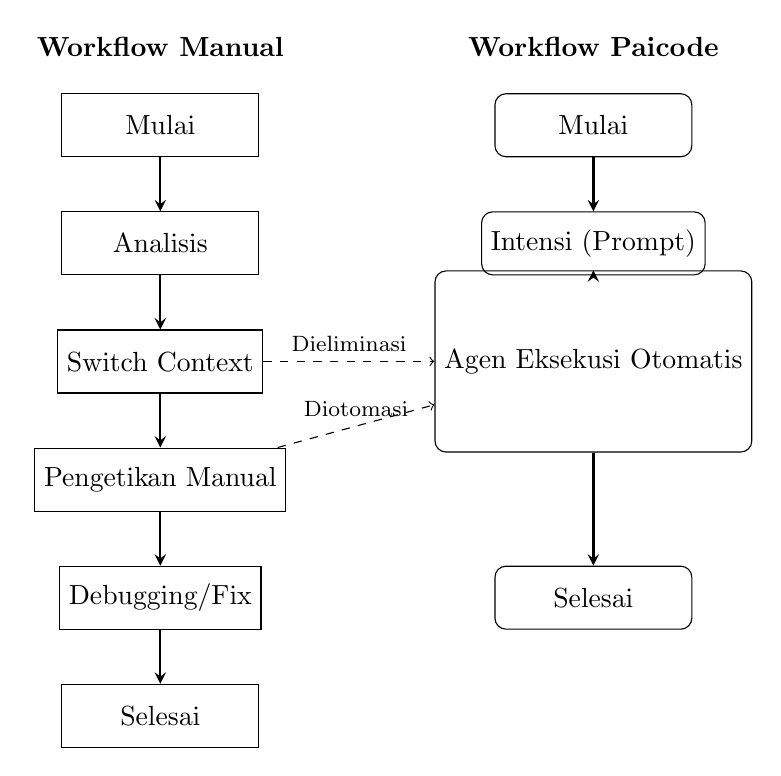
\begin{tikzpicture}[node distance=1.5cm, auto,
    manual/.style={rectangle, draw=black, minimum width=2.5cm, minimum height=0.8cm, text centered},
    agent/.style={rectangle, draw=black, minimum width=2.5cm, minimum height=0.8cm, text centered, rounded corners},
    arrow/.style={thick,->,>=stealth}
  ]
    % Manual Flow
    \node (m_start) [manual] {Mulai};
    \node (m_think) [manual, below of=m_start] {Analisis};
    \node (m_switch) [manual, below of=m_think] {Switch Context};
    \node (m_type) [manual, below of=m_switch] {Pengetikan Manual};
    \node (m_debug) [manual, below of=m_type] {Debugging/Fix};
    \node (m_end) [manual, below of=m_debug] {Selesai};
    
    \draw[arrow] (m_start) -- (m_think);
    \draw[arrow] (m_think) -- (m_switch);
    \draw[arrow] (m_switch) -- (m_type);
    \draw[arrow] (m_type) -- (m_debug);
    \draw[arrow] (m_debug) -- (m_end);
    
    % Agent Flow
    \node (a_start) [agent, right of=m_start, xshift=4cm] {Mulai};
    \node (a_intent) [agent, below of=a_start] {Intensi (Prompt)};
    \node (a_agent) [agent, below of=a_intent, minimum height=2.3cm] {Agen Eksekusi Otomatis};
    \node (a_end) [agent, below of=a_agent, yshift=-1.5cm] {Selesai};
    
    \draw[arrow] (a_start) -- (a_intent);
    \draw[arrow] (a_intent) -- (a_agent);
    \draw[arrow] (a_agent) -- (a_end);
    
    % Labels
    \node [above of=m_start, yshift=-0.5cm] {\textbf{Workflow Manual}};
    \node [above of=a_start, yshift=-0.5cm] {\textbf{Workflow Paicode}};
    
    % Annotation
    \draw [dashed, ->] (m_switch) -- node[above, font=\footnotesize] {Dieliminasi} (a_agent);
    \draw [dashed, ->] (m_type) -- node[above, font=\footnotesize] {Diotomasi} (a_agent);
    
  \end{tikzpicture}
  \caption{Perbandingan alur kerja Manual vs Paicode. Paicode mengeliminasi \textit{context switching} dan beban pengetikan.}
  \label{fig:workflow-comparison}
\end{figure}

\subsection{Keterbatasan Sistem}
Meskipun berhasil memenuhi tujuan utama, sistem masih memiliki keterbatasan:
\begin{enumerate}
    \item Kualitas kode sangat bergantung pada model LLM yang digunakan. Jika API sedang mengalami degradasi layanan, performa agen ikut menurun.
    \item Konteks jendela (\textit{context window}) terbatas. Untuk proyek skala besar dengan ratusan berkas, agen belum bisa "melihat" keseluruhan proyek sekaligus tanpa strategi \textit{retrieval augmented generation} (RAG) yang lebih canggih.
\end{enumerate}
